\subsection{IFIT5} \label{IFIT5}
\subsubsection{Nascent Human and Monkey IFIT5 in a Simplified System of pseudo-IBs} \label{Nascent Human and Monkey IFIT5 in a Simplified System of pseudo-IBs}
\myparagraph{vero hnhp}
Detecting magenta: endogenous monkey IFIT5 \newline
Detecting cyan: human pIB \newline
Cell Line: VERO \newline
Treatment: hNhP \newline

Nascent monkey IFIT5 colocalises with hRSV pseudo inclusion bodies (basically resembling the P staining). It also colocalises with pIB filamentous network. This network is only seen in cells that are co-transfected with RSV N and P proteins. We believe that they are an aftermath of a pIB breakdown. This data is as well supported by z stack measurements.

\begin{figure}
    \centering
    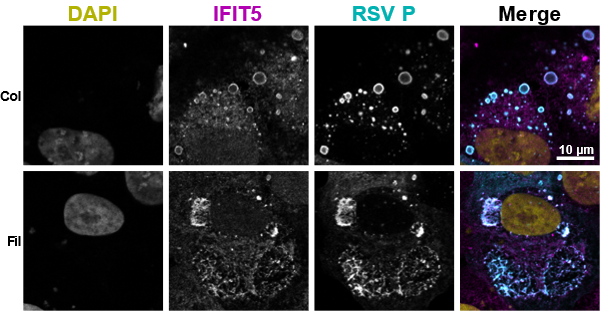
\includegraphics[width=1\linewidth]{08. Chapter 3/Figs/05. IFIT5/01. vero hnhp.png}
    \caption[i5 vero hnhp]{i5 vero hnhp}
    \label{i5 vero hnhp}
\end{figure}

\myparagraph{vero bnbp}
some text

\begin{figure}
    \centering
    
\includegraphics[width=1\linewidth]{06. Chapter 1//Figs/00. placeholder.png}
    \caption[i5 vero bnbp]{i5 vero bnbp}
    \label{i5 vero bnbp}
\end{figure}

\subsubsection{Nascent Human and Bovine IFIT5 Localisation During h/bRSV Infection} \label{Nascent Human and Bovine IFIT5 Localisation During h/bRSV Infection}
\myparagraph{hIFIT5 Localisation During hRSV Infection} \label{hIFIT5 Localisation During hRSV Infection}
\mysubparagraph{a549 hrsv}
Detecting magenta: endogenous human IFIT5 \newline
Detecting cyan: human IB \newline
Cell Line: A549 \newline
Treatment: hRSV \newline

hIFIT5 seems to be excluded from hRSV IBs. There is a hint of accumulation of IFIT5 on the outside of IB (bottom panel; no z stacks to confirm this). 

\begin{figure}
    \centering
    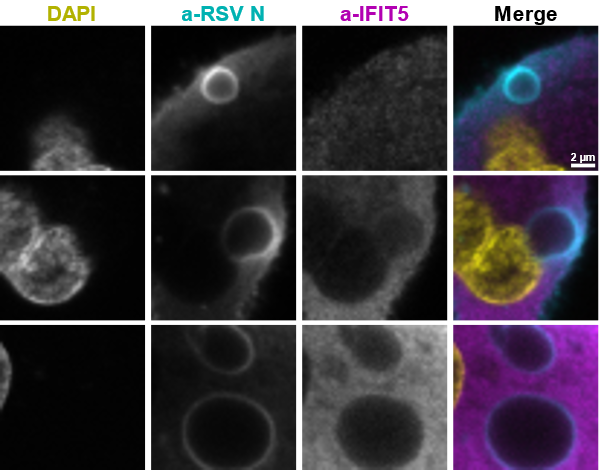
\includegraphics[width=1\linewidth]{08. Chapter 3/Figs/05. IFIT5/02. a549 hrsv.png}
    \caption[i5 a549 hrsv]{i5 a549 hrsv}
    \label{i5 a549 hrsv}
\end{figure}

\mysubparagraph{a549 brsv}
some text

\begin{figure}
    \centering
    
\includegraphics[width=0.5\linewidth]{06. Chapter 1//Figs/00. placeholder.png}
    \caption[i5 a549 brsv]{i5 a549 brsv}
    \label{i5 a549 brsv}
\end{figure}

\mysubparagraph{beas2b hrsv}
Detecting magenta: endogenous human IFIT5 \newline
Detecting cyan: human IB \newline
Cell Line: BEAS2B \newline
Treatment: hRSV \newline

\begin{figure}
    \centering
    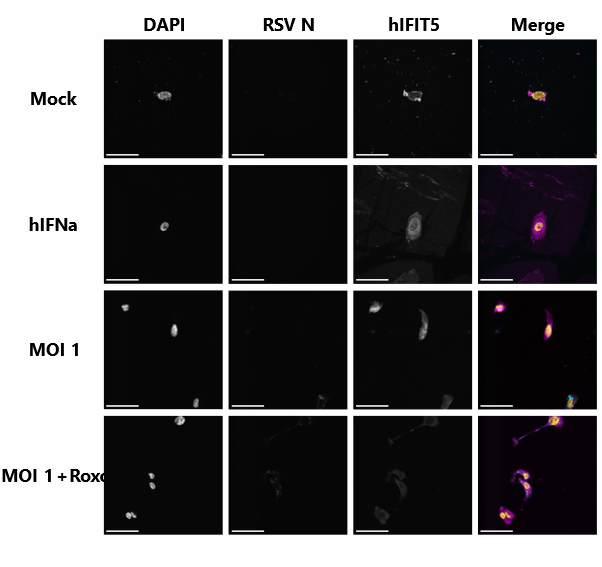
\includegraphics[width=1\linewidth]{08. Chapter 3/Figs/05. IFIT5/03. beas2b hrsv.png}
    \caption[i5 beas2b hrsv]{i5 beas2b hrsv}
    \label{i5 beas2b hrsv}
\end{figure}

\mysubparagraph{beas2b brsv}
some text

\begin{figure}
    \centering
    
\includegraphics[width=0.5\linewidth]{06. Chapter 1//Figs/00. placeholder.png}
    \caption[i5 beas2b brsv]{i5 beas2b brsv}
    \label{i5 beas2b brsv}
\end{figure}

\myparagraph{bIFIT5 Localisation During h/bRSV Infection} \label{bIFIT5 Localisation During h/bRSV Infection}
\mysubparagraph{mdbk hrsv}
some text

\begin{figure}
    \centering
    
\includegraphics[width=0.5\linewidth]{06. Chapter 1//Figs/00. placeholder.png}
    \caption[i5 beas2b brsv]{i5 beas2b brsv}
    \label{i5 beas2b brsv}
\end{figure}

\mysubparagraph{mdbk brsv}
Detecting magenta: endogenous bovine IFIT5 \newline
Detecting cyan: bovine IB \newline
Cell Line: MDBK \newline
Treatment: bRSV dSH + bIFNa \newline

The distribution of bIFIT5 is equal between cytoplasmic stain and inside of the IB (with a hint of concentrations/substructures in top and bottom panel; no z stack data available). All 3 panels show a depression of IFIT5 signal at the side of IB boundary (highlighted by arrows).

\begin{figure}
    \centering
    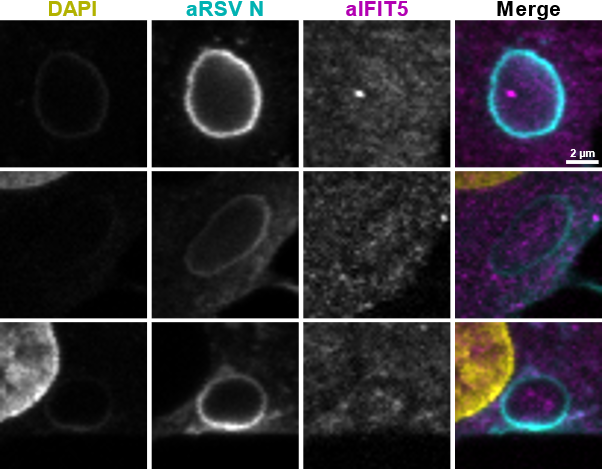
\includegraphics[width=1\linewidth]{08. Chapter 3/Figs/05. IFIT5/04. mdbk brsv.png}
    \caption[i5 mdbk brsv]{i5 mdbk brsv}
    \label{i5 mdbk brsv}
\end{figure}

\mysubparagraph{bt brsv}
some text

\begin{figure}
    \centering
    
\includegraphics[width=0.5\linewidth]{06. Chapter 1//Figs/00. placeholder.png}
    \caption[i5 bt brsv]{i5 bt brsv}
    \label{i5 bt brsv}
\end{figure}

\subsubsection{Exogenously Expressed hIFIT5-FLAG During RSV Infection} \label{Exogenously Expressed hIFIT5-FLAG During RSV Infection}
\myparagraph{hi5 + hrsv brsv}
Detecting magenta: exogenous human IFIT5-FLAG \newline
Detecting cyan: h/bIB \newline
Cell Line: VERO \newline
Treatment: h/bRSV-GFP \newline

hIFIT5-FLAG is colocalising with hRSV inclusion bodies (basically resembling the P staining), while in bRSV infected cell there is a hint of IFIT5 signal concentration at the side of bRSV IB.

This data is by single cells per conditions as transfection did not work well. It is however supported by z stack measurements.


\begin{figure}
    \centering
    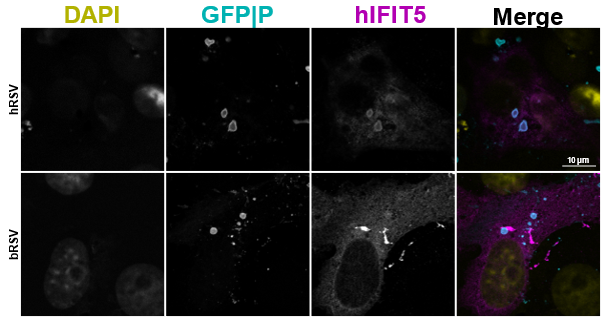
\includegraphics[width=1\linewidth]{08. Chapter 3/Figs/05. IFIT5/05. hi5-hrsv-brsv.png}
    \caption[hi5 + hrsv brsv]{hi5 + hrsv brsv}
    \label{hi5 + hrsv brsv}
\end{figure}

\myparagraph{bi5 + hrsv brsv}
some text

\begin{figure}
    \centering
    
\includegraphics[width=0.5\linewidth]{06. Chapter 1//Figs/00. placeholder.png}
    \caption[bi5 + hrsv brsv]{bi5 + hrsv brsv}
    \label{bi5 + hrsv brsv}
\end{figure}

\subsubsection{Summary} \label{Summary}
Endogenous monkey IFIT5 colocalises with human pIBs and with the NP network (this network is never present in infected cells, so we do not know how are other IFIT5s colocalising with it). In human cells during hRSV infection IFIT5 is mainly excluded from the IBs but seems to concentrate on their edge. Once we saw colocalization with the IB ring and a concentration of IFIT5 inside it. In bovine cells IFIT5 is always excluded from the IB boundary and the signal inside is either slightly decreased or equal compared to cytoplasmic IFIT5. Overexpressed hIFIT5 in hRSV infected cells colocalises with the IBs.